\documentclass[11pt]{article}
\usepackage{times}
\usepackage{amsfonts}
\usepackage{color}
\usepackage{multirow}
%\usepackage{rotating}
\usepackage{url}
\usepackage{latexsym}
\pagenumbering{arabic}
\usepackage{graphicx}
\title{Location-Based Dynamic Social Networks}


\author{
   Vladimir Eidelman, Raul Guerra, and Jim Stevens\\
Department of Computer Science \\
University of Maryland, College Park\\
   %\affaddr{College Park, MD 20742}\\
 { \tt \{vlad,rguerra,jims\}@cs.umd.edu}
}
\begin{document}

\maketitle 

\section{Introduction}


Technology, especially Internet-based technology, has often been portrayed
as having an alienating force by further removing us from `real' social
interaction in favor of the virtual kind. However, a wave of recent
applications has shown that in fact, the opposite can be true. Services
such as Foursquare \cite{foursquare}, Hot Potato \cite{hotp}, and Meetup \cite{meetup} have
shown that we can actually enhance `real' experiences through the use
of technology. In this paper, we present our efforts to extend that line
of thinking in the form of location-based dynamic social networks.

Imagine walking into a classroom or party, and having access to a
dynamic social network with the other people in your immediate area,
including desired profile information and real time information which
is dependent on the venue. Motivated by the previous idea, the Proteus
group implemented an application that generates dynamic networks that are
location dependent for a user to immediately recognize people of interest
and enables a user to establish contact easily with other users. The
main objective is to facilitate interaction with new people around you.
Another objective is to build the location-based service with open tools
and a scalable, general-purpose architecture that is easy to integrate
with already existing services such as Google Maps \cite{google}.
The prototype presented in this paper is the beginning of such a goal and
the future work section will describe how to take the current prototype
to a fully scalable location-based service.

The rest of this paper is structured as follows. First, we will present
our overall system architecture in Section 2, including backend logic,
database interaction, and user interfaces. Then, we will outline the
simulation we developed to test the system in Section 3, followed by a
discussion of future extensions in Section 4.


\section{System Architecture}

\subsection{Overview}

For the user, all interaction with the application takes place through
a web interface. The first interaction users have is creating an
account on the system.  At this point, the user provides their profile
information. A user's profile resembles an online business card, only
containing information they are willing to share with other people,
since the emphasis is not in sharing personal information, but rather
on encouraging real interaction.

To complement the profile information, the user is constantly updating his
or her context information. This includes active updates, in which the user
himself provides additional status information, like a list of interests,
and passive updates (e.g. location) in which the user's information is updated
by the application automatically. The context information, in addition to
the profile, is used by the application to find other users of interest.

The interface interacts with a server to find other nearby users and,
along with their context, displays the network of users logged in at
their locations in a Google Maps interface. Through the Google Map
interface, the user can see other users' real time location, their profile
information, links to other social media, such as Facebook and Twitter,
and have an option to interact with them by either connecting with them
using the social media information or utilizing our graffiti system.

The graffiti system is a way for users to tag certain locations on the 
map with messages. It can be thought of as a tweet at a particular location.
This can enable users to share information with their friends or the entire world,
depending on their privacy settings (note: in the prototype, all graffiti messages
are public). An example use case is to tag a restaurant special or the location
of a party. We also provide an index of graffiti messages to allow users to
easily locate messages they are interested in.

As our application is web-based, it can run on any computer or mobile
device which has a web browser, making it extremely portable. Making
it lightweight in order not to unduly drain the limited resources of
a mobile device was also a design priority, and thus all computation is
performed on the servers, and only the necessary map update process runs
on the device itself.

Previously, achieving such a service on a mobile device required
device-specific code to retrieve the location data from the device. Thanks
to the W3C HTML5 standard \cite{html5}, this is no longer necessary. HTML5
provides a standardized geolocation lookup method that allows browsers
to ask the user to reveal their location to a web application in a
platform independent way. HTML5 geolocation is still in its early stages
of standardization, however, it is expected to be widely deployed in
the near future and as the HTML5 standard becomes more pervasive, this
application will be able to be automatically deployed in any cellphone,
PDA, iPhone, etc. with a  browser supporting HTML5.

%%diagram
Figure ~\ref{fig:arch} shows the structure of our system, as currently implemented. 
The web interface runs in each end user's browser and displays the map
and other aspects of the user interface. The Perl CGI script receives AJAX
HTTP GET requests from the web interface for operations such as update
location or get current output for the user. The MySQL database provides
storage for the system in three tables and provides a way for the modules
to communicate with each other. The User View Daemon takes user session data
as input, updates the user table, and generates JSON output used by the web interface
to display location information to end users. The simulated users represents 
a simulation script that creates a large number of fake users and updates their locations
to allow for large scale system testing.
 
\begin{figure}[h]
\begin{center}
  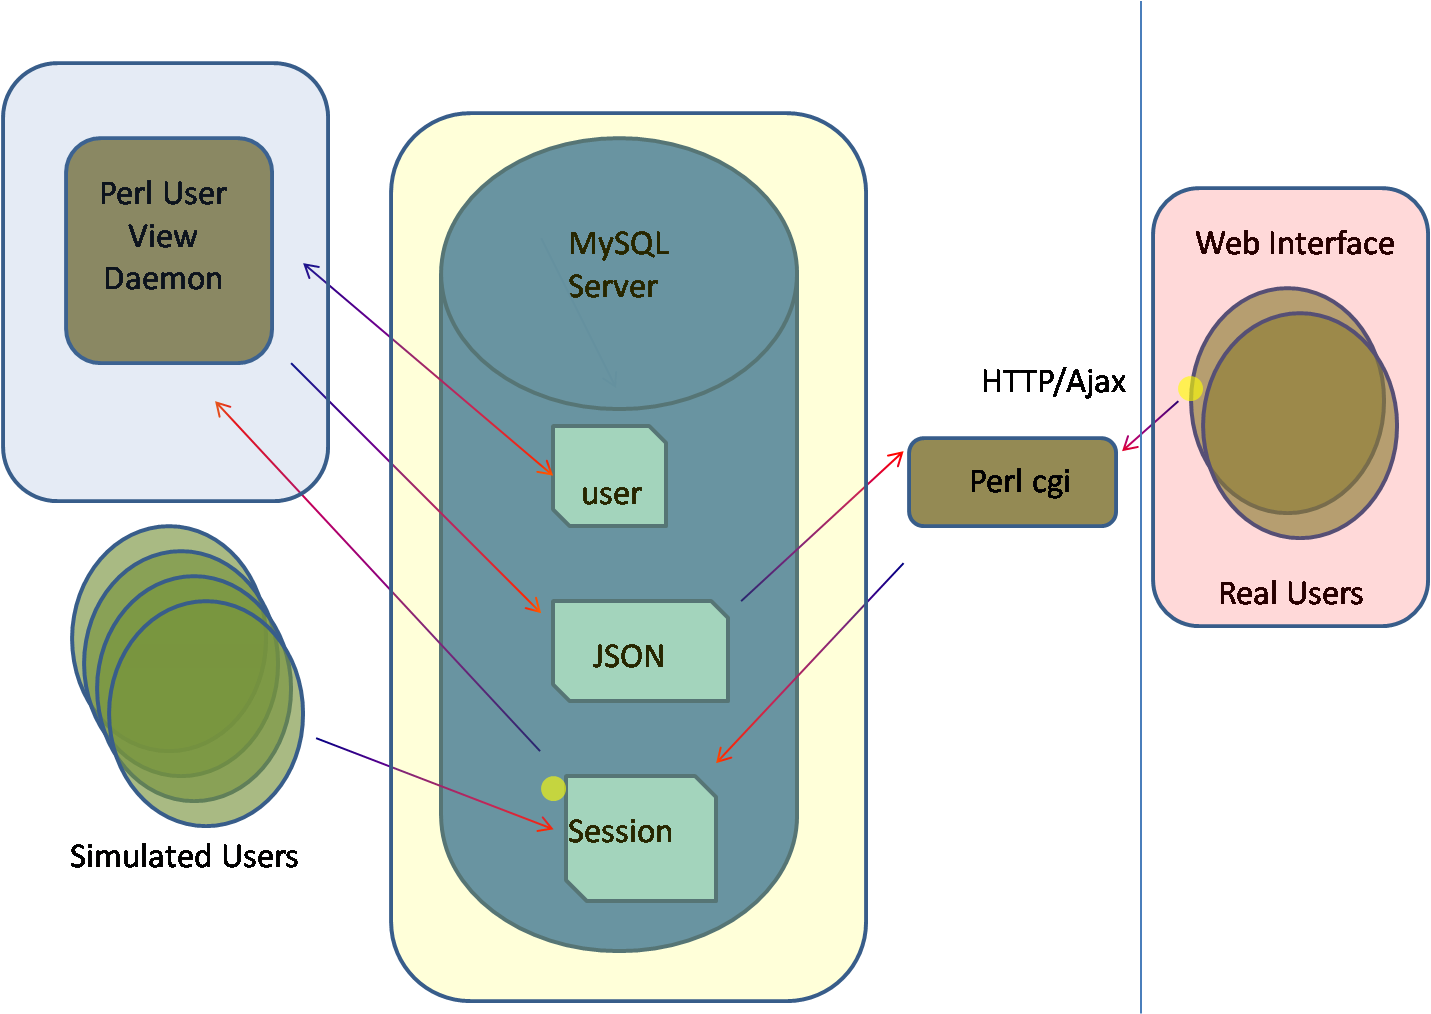
\includegraphics[scale=0.5]{sysarch.png}
\caption{System architecture}
\label{fig:arch} 
\end{center}
\end{figure}



\subsection{Database Setup}

%%database names and descriptions

The MySQL database in this system is used for both interprocess communication
between the system's modules and as a permanent store of user data. The database
currently contains three tables: session, user, and JSON. The basic flow of 
information through the system is that the web interface will insert
records into the session table that correspond to the various types of
updates allowed. The user view daemon will then extract the session records
and use them to update the user table. Finally, the user view daemon will
periodically use the user table information to update the json table, which
contains JSON formatted \cite{json} strings that are interpreted by the web interface
to display location data to the end users.

While using the application, users will enter and leave the dynamic
social network continuously, depending on whether a person is considered
to be active in the network or not. To determine whether a person is
considered to be active, the web interface will send regular updates
to the server. These updates are timestamped, and if the difference
between the timestamp and the current time exceeds a certain value, the
user is considered inactive. When forming the json table entries, only
active users are included. The user table also contains the user's name,
latest location, profile data, and other internal information required
by the server (e.g. if the user is a fake simulated user). Graffiti messages
are also currently stored as user accounts in which the user name is the
message and the location never changes (although this would be refined in
a more mature version of this system).

 

\subsection{User Interface}

The web interface currently support two ways to find information, which
we subsequently describe as location-based and name-based. The two views
compliment each other in that the location view is useful for presenting
a user with the layout of surrounding users, to encourage interaction
with new people in the immediately surrounding area, and the name view
facilitates interacting with already known users. The name view is useful
for quickly browsing Graffiti tags, as opposed to finding all of the
Graffiti tags in the map and clicking one by one to find one of interest.

To implement the location view interface our web
application makes extensive use of Google Maps and its API
(\url{http://code.google.com/apis/maps/documentation/reference.html}).
The API makes it easy to display a Google Map, Graffiti tags, and users,
the last two are just Google Map markers with different icons.

The web interface keeps track of the users that it is currently
displaying, because there are two types of updates it performs. First,
if the web application receives a new user from the  backend server
then it updates the map with a new marker. If it receives an update for
a users it is already displaying then the web application updates the
latitude and longitude of the marker in the map. Having these two type
of updates, as opposed to creating all the users each time it receives
an update, makes the movement of the users in the map much smoother due
to lower processor usage. This increases the memory overhead of the web
application only slightly. As mentioned above a user through the web
application sends continuous updates to indicate the he or she is still
active. Thus an inactive user is one that is not continuously updating
its location. These type of users are no longer present in the social
network or inactive. When this happens the backend server stops sending
information about a user and the web application stops displaying him
or her in both the Map and the names list. A pause/play button is also
provided to allow the user to pause the map updates to make it easier to
click on a particular user that may be moving. Figure ~\ref{fig:phoneapp}
shows the proposed interface for a mobile device.


\begin{figure}[h]
\begin{center}
  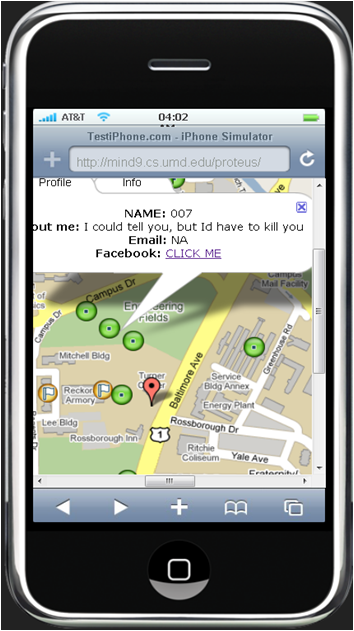
\includegraphics[scale=0.5]{phoneapp.png}
\caption{Example Apple iphone interface}
\label{fig:phoneapp} 
\end{center}
\end{figure}



\subsubsection{Graffiti/Tagging}

The Graffiti capability comes from the concept of social tagging
and the idea of personalizing a place for the duration of the dynamic
social network. This functionality allows users to actively comment
on the particular venue and input information into the web
application system that could be used for a variety of purposes. One possibility is
that a recommendation engine could use this input and match users whose
Graffiti behavior is similar. Another is using the Graffiti information
to try to predict a user's behavior. For example, if a user has posted
negative Graffiti in a restaurant, the web application can take this
into account next time it recommends a place to eat. The final example
is that Graffiti can be used as an indirect way of communicating. The
Graffiti can be a forum where lots of users post messages. However,
Graffiti differs from forums because it is transient and it only exists
for the duration of dynamic social network. Thus, Graffiti more closely
resembles a group of people gathering at a place to gossip than a forum.

Currently Graffiti is the only way for users to communicate through the
web application. As mentioned before to do this a user leaves messages
at specific locations and other users can see these messages and leave
their own.

\subsubsection{Business Card/Profile}

For the purpose of keeping the prototype of the system simple, we
assumed that all users trust each other with their profile data.  Therefore,
the system does not currently support anonymous users and each user has 
a profile with his or her information on it and shares it with others. 
Since the purpose of the web application is not to keep a
repository of information for each user like Facebook, and our application
seeks to facilitate social interaction among users, the profiles are
slim and provide just enough information for a user to identify and contact
the user using email or other social networks.

\subsection{CGI Script}

The CGI script runs as the server side complement to the user interface.
It processes AJAX HTTP GET requests from the user interface and interacts
with the MySQL database to either insert records into the session table
or retrieve records from the json table.

\subsection{Daemon}

The user view daemon runs in the background to maintain the database.
It is the backend component of the system that facilitates communication
between all users.  The daemon runs once per second and operates in three
stages. First, it reads all records from the session table and updates
the user table with the new locations, profile updates, graffiti,
etc. Second, the user table is checked for expired users, which if
found are marked inactive.  Third, for each active non-simulated user,
a JSON-formatted string is generated and placed in the json table for
that user to later retrieve and display.


\section{Simulation}


In order to both validate the concept of our system and assess the
structural limitations, we were inclined to design a simulation wherein we
created virtual users. Utilizing the modularity described above, we were
able to create an additional program which generated virtual users and
updated their location, as if they were walking around campus, and plug it
into our existing system as if the upates were coming in from real users.

The program generates 25 virtual users in random locations within
College Park, along with their profile information, which includes
emails and Facebook links. Then the program assigns one of 16 possible
destinations for each user, and moves each user at a random reasonable
rate toward their chosen destination, updating the appropriate tables
in the database at the normal time intervals. The list of possible
destinations includes itesm such as AV Williams, Stamp Student Union,
the library, and downtown. Once a user reaches the assigned destination,
a new one is chosen for them at random and the simulation proceeds.

While the simulation is active, a real user can log into the system
and interact with any one of the virtual users. Using the simulation
provided us with a convenient way of presenting our vision for
what the real application interface would feel like, as depicted in
Figure~\ref{fig:sim1}.


\begin{figure}[h]
\begin{center}
  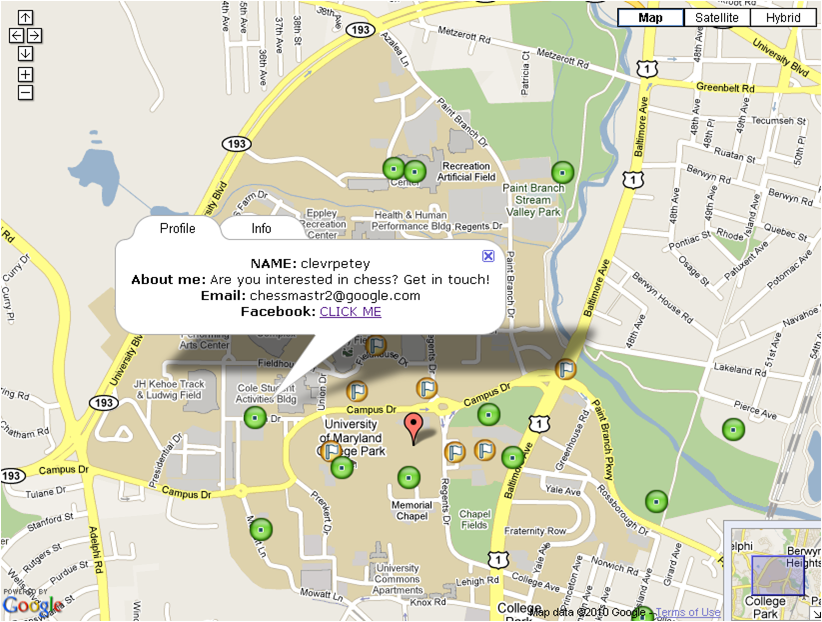
\includegraphics[scale=0.5]{sim1.png}
\caption{Example Simulation}
\label{fig:sim1} 
\end{center}
\end{figure}



\section{Future Work}

The goal of this project was to develop a design for a system that could
actually be deployed and used by millions of users. To take the current 
prototype and create such a system, two issues need to be addressed:
additional features and preparing for very large scale use. 

The additional features needed in this system are rather minor. First,
we would want to add in privacy features such as anonymous business cards
and limited location knowledge (e.g. a user may reveal the city they
are in, but not the exact address). Second, a powerful recommendation
engine such as one used by Amazon or Netflix is desirable to help focus
users on certain types of conetent and connect them with users that match
their interests.  Third, complete integration with other social networks
such as Twitter and Facebook and instant message clients such as GTalk
or AIM is desirable to enable users to immediately communicate upon
contacting each other. We do not feel these features should be directly
implemented in this system because they already exist elsewhere and this
system intends to simply facilitate connecting users based on location,
not providing the actual communication channel.

The main scalability issue that needs to be addressed is the potential
for server overload. We believe the appropriate design is to divide
the world into a quadtree-like grid and then have one server service
each quadtree leaf node. This technique is how many geographic systems currently
achieve scalability.  For robustness, when users connect to the system
they will connect to the server that covers their area as well as several
nearby servers. The servers will then update their neighbors in case one
goes down. As users move around, they will be handed off from server to
server. As users and servers are added to or removed from the system, the quadtree
can be subdivided, combined, or reorganized based on the local load needs
(e.g. NYC will have many servers but rural areas such as the midwest will
have few). The scability issue is obviously very deep, but we believe this
basic grid-based design will suffice for even very large social networks
such as the Facebook user base. The reason is because all communication
in such a system stays local between the neighbor servers and overloaded
servers are automatically split up to load balance.


\section{Conclusion}

In this paper we have presented a prototype for a scalable location-based
service using open standards and open tools such as HTML5, MySQL, and
Google Maps.  Although this is not the first location-based service,
we believe that this project provides unique utility due to the simple,
scalable, and modular design as well as novel features such as the
graffiti messages and simple business card to encourage interaction among
strangers. This web application gives a new perspective to Heraclitus's
(c. 500 B.C.) famous saying "One can't step into the same river twice,
since the river never remains the same" by updating it to "One cannot
visit the same dynamic social network twice, since a social dynamic
network never remains the same users constantly enter and leave".


\bibliographystyle{abbrv}
\bibliography{references}

\end{document}



